%% March 2018
%%%%%%%%%%%%%%%%%%%%%%%%%%%%%%%%%%%%%%%%%%%%%%%%%%%%%%%%%%%%%%%%%%%%%%%%%%%%
% AGUJournalTemplate.tex: this template file is for articles formatted with LaTeX
%
% This file includes commands and instructions
% given in the order necessary to produce a final output that will
% satisfy AGU requirements, including customized APA reference formatting.
%
% You may copy this file and give it your
% article name, and enter your text.
%
%
% Step 1: Set the \documentclass
%
% There are two options for article format:
%
% PLEASE USE THE DRAFT OPTION TO SUBMIT YOUR PAPERS.
% The draft option produces double spaced output.
%

%% To submit your paper:
\documentclass[draft]{agujournal2018}
\usepackage{apacite}
\usepackage{textcomp}
\usepackage{url} %this package should fix any errors with URLs in refs.
\usepackage{lineno}
%\linenumbers
%%%%%%%
% As of 2018 we recommend use of the TrackChanges package to mark revisions.
% The trackchanges package adds five new LaTeX commands:
%
%  \note[editor]{The note}
%  \annote[editor]{Text to annotate}{The note}
%  \add[editor]{Text to add}
%  \remove[editor]{Text to remove}
%  \change[editor]{Text to remove}{Text to add}
%
% complete documentation is here: http://trackchanges.sourceforge.net/
%%%%%%%

\draftfalse

%% Enter journal name below.
%% Choose from this list of Journals:
%
% JGR: Atmospheres
% JGR: Biogeosciences
% JGR: Earth Surface
% JGR: Oceans
% JGR: Planets
% JGR: Solid Earth
% JGR: Space Physics
% Global Biogeochemical Cycles
% Geophysical Research Letters
% Paleoceanography and Paleoclimatology
% Radio Science
% Reviews of Geophysics
% Tectonics
% Space Weather
% Water Resources Research
% Geochemistry, Geophysics, Geosystems
% Journal of Advances in Modeling Earth Systems (JAMES)
% Earth's Future
% Earth and Space Science
% Geohealth
%
% ie, \journalname{Water Resources Research}

\journalname{JGR: Solid Earth}


\begin{document}

%% ------------------------------------------------------------------------ %%
%  Title
%
% (A title should be specific, informative, and brief. Use
% abbreviations only if they are defined in the abstract. Titles that
% start with general keywords then specific terms are optimized in
% searches)
%
%% ------------------------------------------------------------------------ %%

% Example: \title{This is a test title}

\title{Primary and secondary red bed magnetization constrained by fluvial intraclasts}

%% ------------------------------------------------------------------------ %%
%
%  AUTHORS AND AFFILIATIONS
%
%% ------------------------------------------------------------------------ %%

% Authors are individuals who have significantly contributed to the
% research and preparation of the article. Group authors are allowed, if
% each author in the group is separately identified in an appendix.)

% List authors by first name or initial followed by last name and
% separated by commas. Use \affil{} to number affiliations, and
% \thanks{} for author notes.
% Additional author notes should be indicated with \thanks{} (for
% example, for current addresses).

% Example: \authors{A. B. Author\affil{1}\thanks{Current address, Antartica}, B. C. Author\affil{2,3}, and D. E.
% Author\affil{3,4}\thanks{Also funded by Monsanto.}}

\authors{Nicholas L. Swanson-Hysell\affil{1}, Luke M. Fairchild\affil{1}, Sarah P. Slotznick\affil{1}}


% \affiliation{1}{First Affiliation}
% \affiliation{2}{Second Affiliation}
% \affiliation{3}{Third Affiliation}
% \affiliation{4}{Fourth Affiliation}

\affiliation{1}{Department of Earth and Planetary Science, University of California, Berkeley, CA, USA}
%(repeat as many times as is necessary)

%% Corresponding Author:
% Corresponding author mailing address and e-mail address:

% (include name and email addresses of the corresponding author.  More
% than one corresponding author is allowed in this LaTeX file and for
% publication; but only one corresponding author is allowed in our
% editorial system.)

% Example: \correspondingauthor{First and Last Name}{email@address.edu}

\correspondingauthor{Nicholas Swanson-Hysell}{swanson-hysell@berkeley.edu}

%% Keypoints, final entry on title page.

%  List up to three key points (at least one is required)
%  Key Points summarize the main points and conclusions of the article
%  Each must be 100 characters or less with no special characters or punctuation

% Example:
% \begin{keypoints}
% \item	List up to three key points (at least one is required)
% \item	Key Points summarize the main points and conclusions of the article
% \item	Each must be 100 characters or less with no special characters or punctuation
% \end{keypoints}

\begin{keypoints}
\item Red siltstone intraclasts reveal two ancient magnetizations held by hematite -- one acquired before redeposition and the other after burial
\item Fine-grained hematite spans from superparamagnetic to single domain leading to a wide range of unblocking temperatures and coercivities
\item  Detrital hematite thermally unblocks in a narrow high temperature range that can be isolated through high-resolution thermal demagnetization


\end{keypoints}

%% ------------------------------------------------------------------------ %%
%
%  ABSTRACT
%
% A good abstract will begin with a short description of the problem
% being addressed, briefly describe the new data or analyses, then
% briefly states the main conclusion(s) and how they are supported and
% uncertainties.
%% ------------------------------------------------------------------------ %%

%% \begin{abstract} starts the second page

\begin{abstract}

The magnetization of hematite-bearing sedimentary rocks provides critical records of geomagnetic reversals and paleogeography. However, the timing of hematite remanent magnetization acquisition is typically difficult to constrain. While detrital hematite in sediment can lead to a primary depositional remanent magnetization, alteration of minerals through interaction with oxygen can lead to the post-depositional formation of hematite. In this study, we use exceptionally-preserved fluvial sediments within the 1.1 billion-year-old Freda Formation to gain insight into the timing of hematite remanence acquisition and its magnetic properties. This deposit contains siltstone intraclasts that were eroded from a coexisting lithofacies and redeposited within channel sandstone. Thermal demagnetization, petrography and rock magnetic experiments on these clasts reveal two generations of hematite. One population of hematite demagnetized at the highest unblocking temperatures and records directions that rotated along with the clasts. This component is a primary detrital remanent magnetization. The other component is removed at lower unblocking temperatures and has a consistent direction throughout the intraclasts. This component is held by finer-grained hematite that grew and acquired a chemical remanent magnetization following deposition resulting in a population that includes superparamagnetic nanoparticles in addition to remanence-carrying grains. The data support the interpretation that magnetizations of hematite-bearing sedimentary rocks held by $>$400 nm grains that unblock close to the N\'eel temperature are more likely to record magnetization from the time of deposition. This primary magnetization can be successfully isolated from co-occurring authigenic hematite through high-resolution thermal demagnetization.

\end{abstract}



%% ------------------------------------------------------------------------ %%
%
%  TEXT
%
%% ------------------------------------------------------------------------ %%

%%% Suggested section heads:
% \section{Introduction}
%
% The main text should start with an introduction. Except for short
% manuscripts (such as comments and replies), the text should be divided
% into sections, each with its own heading.

% Headings should be sentence fragments and do not begin with a
% lowercase letter or number. Examples of good headings are:

% \section{Materials and Methods}
% Here is text on Materials and Methods.
%
% \subsection{A descriptive heading about methods}
% More about Methods.
%
% \section{Data} (Or section title might be a descriptive heading about data)
%
% \section{Results} (Or section title might be a descriptive heading about the
% results)
%
% \section{Conclusions}


\section{Introduction}

The magnetizations of hematite-bearing sedimentary rocks known as ``red beds'' have provided ample opportunities for Earth scientists to gain insight into the ancient geomagnetic field and the paleogeographic positions of sedimentary basins. However, with these opportunities has come much scientific debate, leading to what has been referred to as the ``red bed controversy'' \citep{Butler1992a, Beck2003b, Van-Der-Voo2012a}. This controversy stems from the reality that hematite within sedimentary rocks can have two sources: 1) detrital grains that are within the sediment at the time of deposition; 2) grains that grow \textit{in situ} after the sediments have been deposited.

How does one constrain the relative age of hematite within sedimentary rocks? Many of the traditional paleomagnetic field tests are unable to differentiate between primary versus diagenetic remanence. For example, a structural fold test can constrain that a remanence direction was obtained prior to folding, but millions of years have typically passed between the deposition of a sediment and such tectonic tilting. Dual-polarity directions through a sedimentary succession are commonly interpreted as providing assurance that the remanence records primary or near-primary magnetization; however, hematite growth could occur significantly after deposition during a protracted period over which the geomagnetic field was in both reversed and normal polarities. Petrographic investigations are valuable, but it can be difficult to ascertain how much the petrographically observed hematite contributes to the magnetization and to unambiguously interpret whether observed grains are detrital or not (e.g. \citealp{Elmore1982a}). A common approach to classify hematite grains within red beds is into a fine-grained pigmentary population, typically interpreted to have formed within the sediment, and a coarser-grained population that has been referred to in the literature as ``specularite'' \citep{Butler1992a, Van-Der-Voo2012a}. \citet{Tauxe1980a} showed that sediments with abundant red pigmentary hematite in the Miocene Siwalik Group had lower thermal unblocking temperatures than grey samples dominated by a coarser-grained phase of specular hematite. An additional approach taken by \citet{Tauxe1980a}, and other workers going back to the work of \citet{Collinson1965a}, is to preferentially remove fine-grained pigmentary hematite through prolonged immersion in concentrated HCl acid. Paired chemical and thermal demagnetization have been interpreted to show that removal of pigmentary hematite coincides with removal of hematite associated with lower unblocking temperatures. These data support the interpretation that coarser grains that are more resistant to dissolution in acid correspond with those that carry remanence to the highest unblocking temperatures \citep{Tauxe1980a,Bilardello2010c}; although simultaneous dissolution of fine and coarser hematite can occur \citep{Jiang2017a}. Observations such as these have led to the practice of defining the characteristic remanent magnetization from hematite-bearing sediments as that held by the highest unblocking temperatures \citep{Van-Der-Voo2012a}. Additional lines of evidence in numerous successions have supported this approach. For example, in the well-studied Carboniferous Mauch Chunk Formation of Pennsylvania, remanence removed up to $\sim$660\textdegree C has uniform polarity and fails a fold test while the component removed upwards of 670\textdegree C is dual-polarity, was acquired before folding, and is interpreted as a primary magnetization \citep{Kent1985b, DiVenere1991a}. Nevertheless, the primary versus secondary nature of micron-scale ``specularite'' grains that likely carry this remanence has been one of the largest sources of contention in the ``red bed controversy'' \citep{Van-Houten1968a, Tauxe1980a, Butler1992a, Van-Der-Voo2012a}.

What is needed to most confidently address the timing of remanence acquisition is a process that reorients the sediment before it has been lithified. Two such processes are: 1) syn-sedimentary slumping wherein coherent sediment is reoriented through soft-sediment folding in the surface environment and 2) intraclasts comprised of the lithology of interest that have been liberated and redeposited within the depositional environment. Sediments that have undergone reorienting processes within the depositional environment can provide significant insight into whether magnetization was acquired before or after reorientation.

\citet{Tauxe1980a} studied 7 cobble-sized clasts within the Siwalik Group that were interpreted to have formed by cut-bank collapse and discovered that their magnetic remanence was acquired prior to clast reorientation. \citet{Molina-Garza1991a} observed dispersed magnetization directions in sandstone and siltstone clasts within the Triassic Moenkopi and Chinle formations in New Mexico and interpreted the characteristic remanence to be a detrital or early chemical remanence. An investigation by \citet{Purucker1980a} on red beds also of the Triassic Moenkopi Formation of Arizona used multiple such syn-sedimentary processes to gain insight into hematite acquisition. In their study, an intraformational landslide deposit with isoclinal folds of hematite-bearing claystone revealed non-uniform directions upon blanket demagnetization to 650\textdegree C that cluster better when corrected for their tilt, leading to a primary interpretation for their remanence. Scatter was also observed in intraformational conglomerate clasts weathered out of an underlying unit upon blanket thermal demagnetization to 630\textdegree C. However, the lack of principal component analysis makes it difficult to evaluate the coherency of the directions. Complicating matters, \citet{Larson1982b} analyzed shale rip-up clasts in the same Moenkopi Formation and used the fact that similar remanence directions were removed between clasts during thermal demagnetization up to 645\textdegree C as support for the hypothesis that red beds rarely reflect the geomagnetic field at the time of deposition. Evaluating the robustness of this result, as well as the varying results of similar field tests conducted by \citet{Liebes1982a} on the Chugwater and Moenkopi formations, is hindered by the cessation of thermal demagnetization before the N\'eel temperature of hematite and the lack of principal component analysis. These limitations are found in many studies from this era of research, when the red bed controversy was particularly fervent, as the work predates the widespread application of principal component analysis in conjunction with systematic progressive thermal demagnetization \citep{Kirschvink1980a, Van-Der-Voo2012a}. Using such methods, \citet{Opdyke2004a} analyzed 20 red siltstone rip-up clasts from the Mauch Chunk Formation and found that the remanence component that unblocks above 650 \textdegree C and passes a structural fold test was reoriented with the rip-up clasts providing strong evidence for a syndepositional or early post-depositional origin of the hematite.

In this study, we investigate cm-scale siltstone intraclasts within the ca. 1.1 Ga Freda Formation that were eroded by fluvial processes and redeposited amongst cross-stratified sandstones (Fig. \ref{fig:intraclast_images}). High-resolution thermal demagnetization data on these clasts constrain the timing of hematite acquisition by revealing a primary component that formed prior to the erosion of the clasts within the depositional environment and a secondary component that formed following their redeposition. Rock magnetic experiments constrain the magnetic mineralogy and provide additional insights into the grain size of the hematite populations that hold these remanences.

\begin{figure}[!ht]
\centering
\noindent\includegraphics[width=\textwidth]{figures/BRIC_clast_images_2.png}
\caption{\small{A: Siltstone intraclasts within the Freda Formation. The field photo shows an intact layer of siltstone below the hammer head which is topped by a bed of trough cross-stratified coarse-grained sandstone with horizons of siltstone intraclasts. The hammer is 40 cm long. The inset photo is of an individual intraclast that was sampled as BRIC.26. B: A scan of a thin section of the BRIC.26 intraclast (upper half of image) and the coarse sand matrix (lower half of image). The red color of the intraclast is due to pigmentary hematite. C: Backscatter electron image of the siltstone clast from the region of the white box in B. The light-colored detrital grains that are labeled with arrows (light due to iron's high atomic number) were confirmed to be hematite through electron backscatter diffraction.}}
\label{fig:intraclast_images}
\end{figure}

The $\sim$5 km thick Freda Formation was deposited in the North American Midcontinent Rift as it was thermally subsiding following the cessation of widespread magmatic activity \citep{Cannon1992b}. The fluvial sediments of the Freda Formation are part of the Oronto Group and were conformably deposited following the deposition of the alluvial Copper Harbor Conglomerate and the lacustrine Nonesuch Formation \citep{Ojakangas2001a, Slotznick2018b}.  Abundant fine-grained red siltstones within the Freda Formation have a well-behaved magnetic remanence dominated by hematite \citep{Henry1977a}. A maximum age constraint on the Freda Formation of 1085.57 $\pm$ 0.25/1.3 Ma (2$\sigma$ analytical/analytical + tracer + decay constant uncertainty; \citealp{Fairchild2017a}) is provided by an U-Pb date of a lava flow within the underlying Copper Harbor Conglomerate. Minor volcanics within the Freda Formation on the Keweenaw Peninsula are unlikely to be substantially younger than the youngest dated volcanics within the Midcontinent basin (1083.52 $\pm$ 0.23/1.2 Ma from the Michipicoten Island Formation; \citealp{Fairchild2017a}). An age of ca. 1080 Ma for the basal 500 meters of the Freda Formation is consistent with modeling of post-rift thermal subsidence \citep{Hutchinson1990a}.

The studied intraclast-bearing outcrop is located along the Bad River (northern Wisconsin) in the lower portion of the Freda Formation -- approximately 320 to 340 meters above its conformable base with the Nonesuch Formation (latitude:  46.3866 \textdegree N, longitude 90.6373 \textdegree W). The two main lithofacies in the studied outcrop are: (1) siltstone to very fine sandstone with planar lamination and horizons of ripple cross-stratification and (2) coarse to very coarse subarkosic sandstone with dune-scale trough cross-stratification (Fig. \ref{fig:intraclast_images}). These lithofacies are consistent with a fluvial depositional environment where the coarse sandstone facies are channel deposits and the siltstones are inner-bank or over-bank deposits. The coarse-grained sandstone contains horizons of tabular cm-scale intraclasts comprised of the red siltstone lithology that is present in underlying beds of intact siltstone (Fig. \ref{fig:intraclast_images}). These tabular clayey-silt intraclasts were eroded within the depositional environment and redeposited in the sandstone. Due to migrating channels in fluvial systems, it is expected that a river will erode its own sediments. The intraclasts would have been held together through cohesion resulting from the clay component within the sediment. Given that the clasts are large (1 to 7 cm) relative to their host sediment, that they are angular, and that they would have been fragile at the time of deposition, it is unlikely that they were transported far within the channel.

\section*{Paleomagnetic Results}

Oriented samples were collected and analyzed from 39 Freda Formation intraclasts. The dimensions of the sampled clasts ranged from 2.2 x 1.4 x 0.5 cm to 7.2 x 2.3 x 1.2 cm. Given that the clasts were typically smaller than the 1-inch-diameter drill cores used for sampling, they were collected along with their sandstone matrix. These oriented cores were mounted onto quartz glass discs with Omega CC cement and the matrix material was micro-drilled away. The mounted clasts underwent stepwise thermal demagnetization in the UC Berkeley Paleomagnetism Lab using an ASC demagnetizer (residual fields $<$10 nT) with measurements made on a 2G DC-SQUID magnetometer. The demagnetization protocol had high resolution  approaching the Ne\'el temperature of hematite (5\textdegree C to 2\textdegree C to 1\textdegree C) resulting in 30 total thermal demagnetization steps (Fig. \ref{fig:intraclast_pmag}). All paleomagnetic data are available to the measurement level in the MagIC database (\url{https://earthref.org/MagIC/doi/}). \textit{So that reviewers have access to the data, they are currently available in CIT lab format and MagIC format here: \url{https://github.com/Swanson-Hysell-Group/2018_Red_Bed_Intraclasts}}.

\begin{figure}[!ht]
\noindent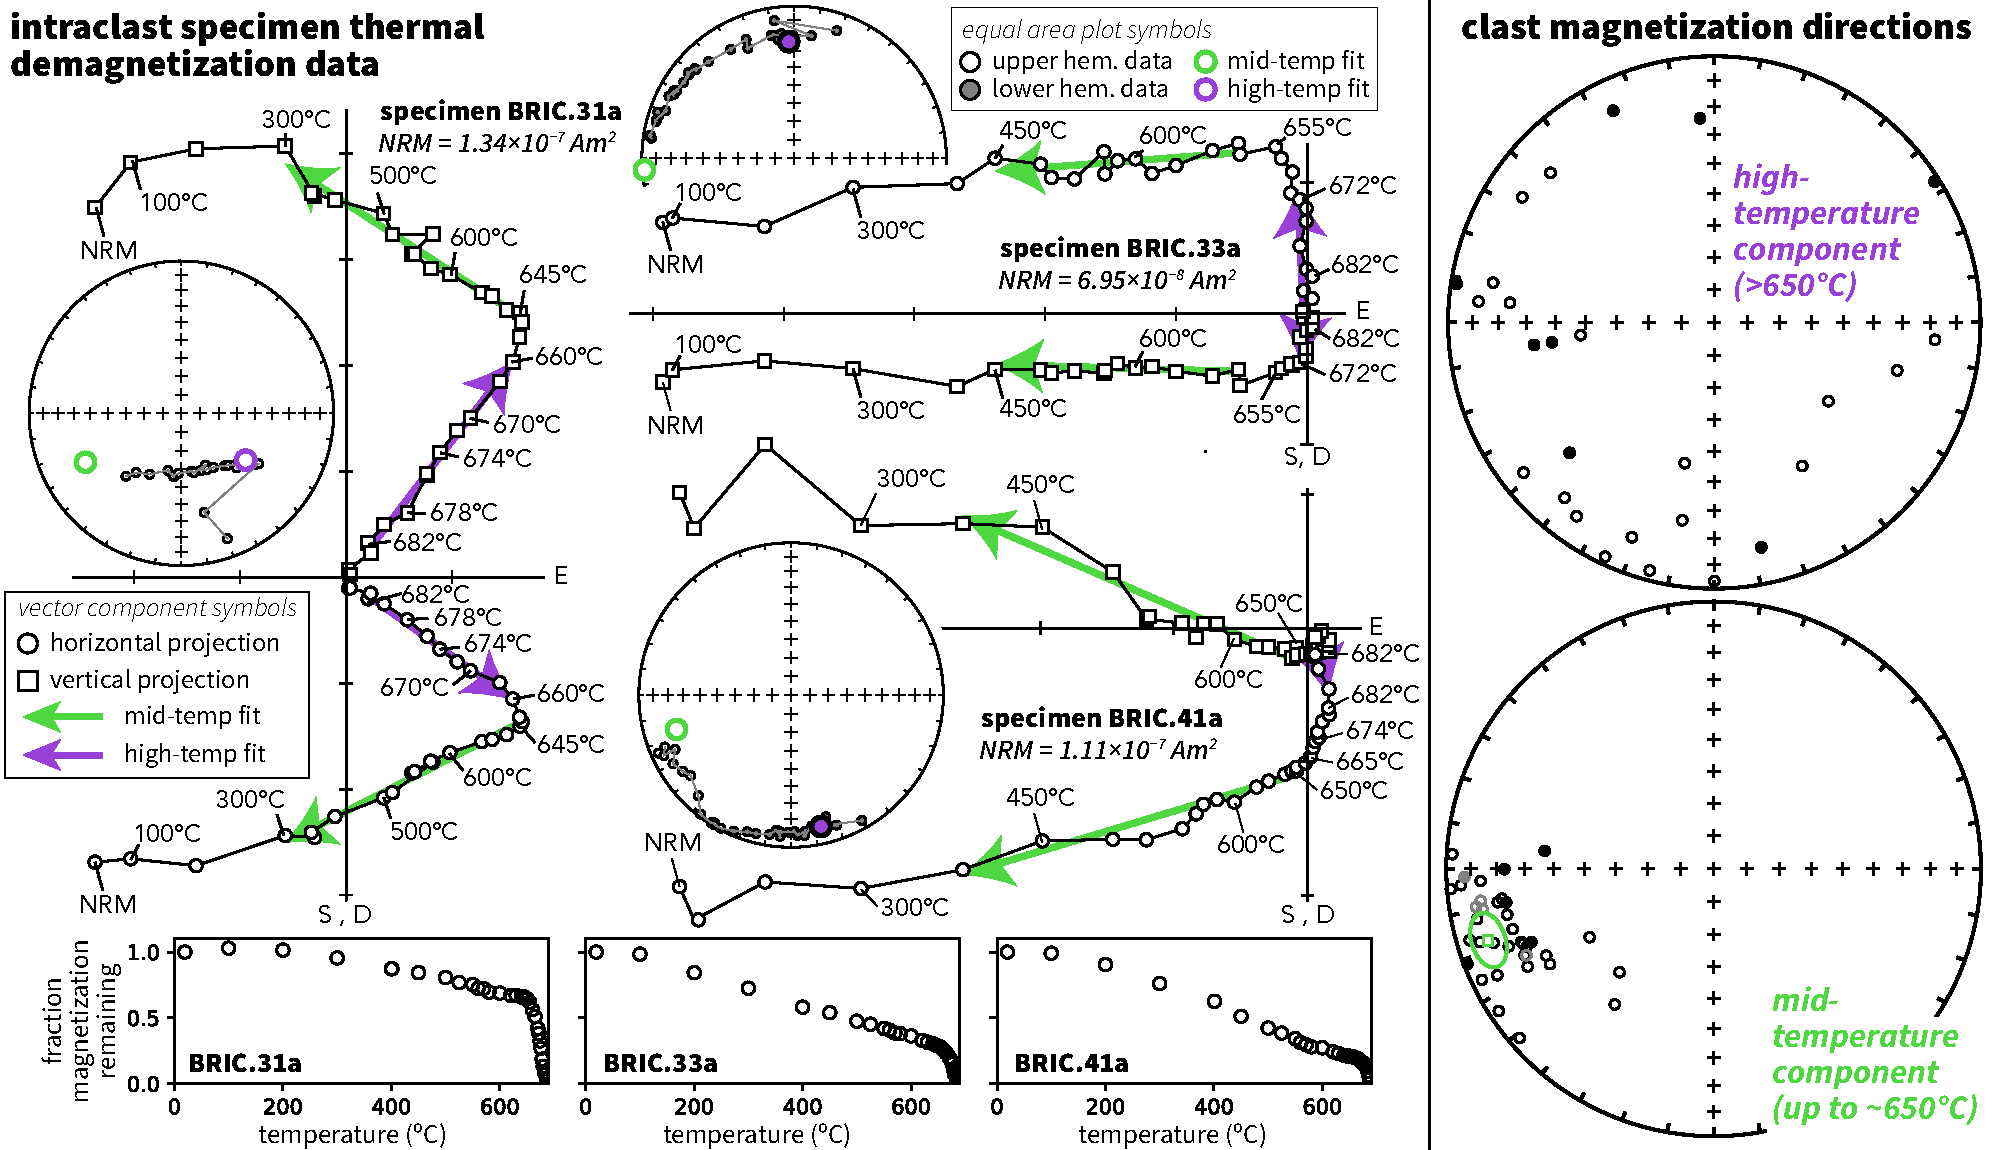
\includegraphics[width=\textwidth]{figures/BRIC_pmag.pdf}
\caption{\small{Paleomagnetic data from intraclasts reveal a mid-temperature component that typically unblocks prior to 655\textdegree C and a high-temperature component that typically unblocks between 655\textdegree C and 687\textdegree C. These components are present as varying fractions of the overall remanence as seen in the three individual clasts shown here on vector component plots and measurement-level equal area plots in tilt-corrected coordinates (developed using PmagPy; \citealp{Tauxe2016a}). The direction of the mid-temperature component is shown as green arrows on the vector component plots and green circles on the equal area plots while the high-temperature component is shown with purple symbols. The mid-temperature component has a similar direction among the clasts as can be seen on the component directions equal area plots (tilt-corrected mean declination: 252.4, inclination: -12.5, $\alpha_{95}$: 6.6). In contrast, the high-temperature component directions are dispersed.}}
\label{fig:intraclast_pmag}
\end{figure}

\begin{figure}[!ht]
\noindent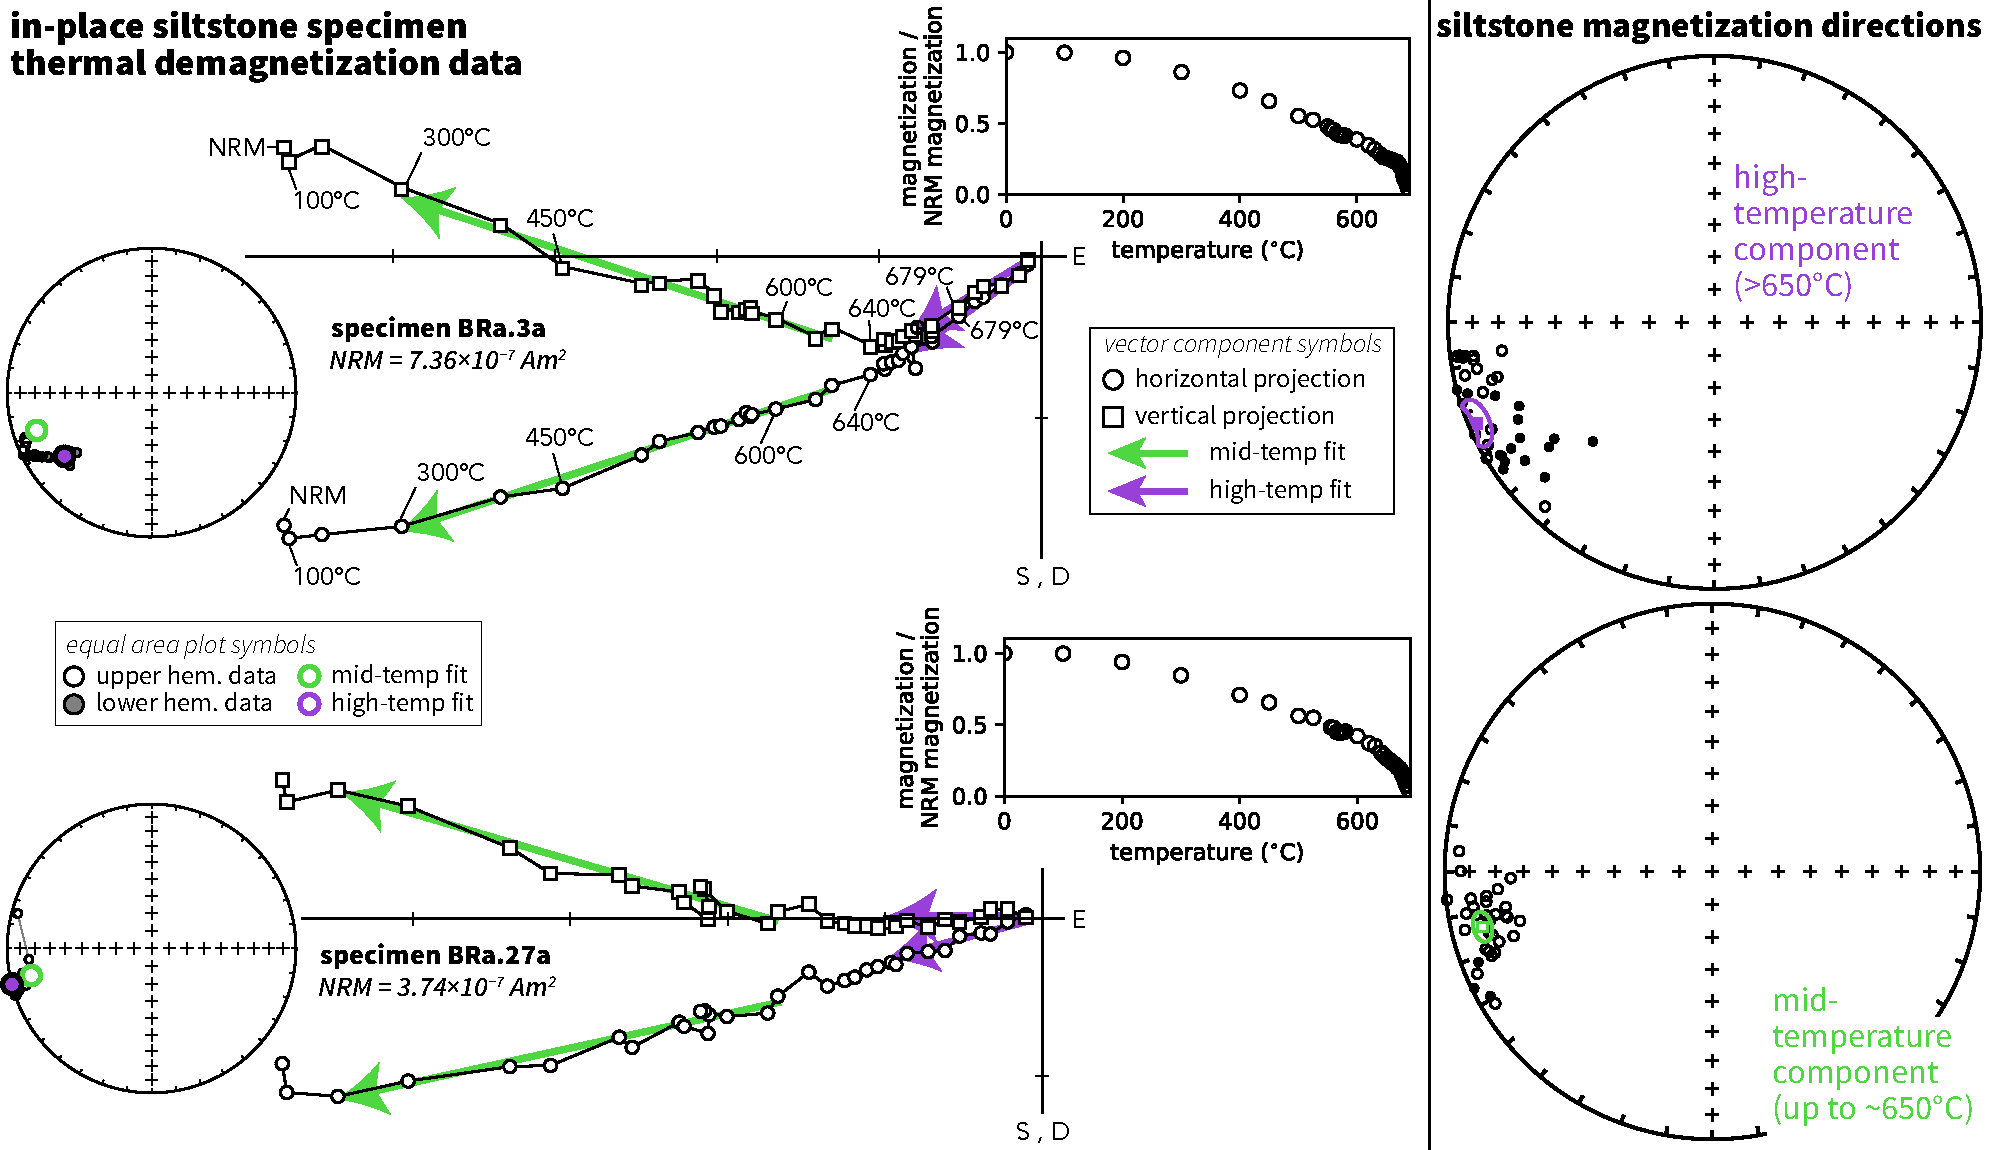
\includegraphics[width=\textwidth]{figures/BRa_pmag.pdf}
\caption{\small{Paleomagnetic data from in-place siltstone beds reveal a mid-temperature component that typically unblocks prior to 655\textdegree C and a high-temperature component that typically unblocks between 655\textdegree C and 689\textdegree C. The direction of the mid-temperature component is shown as purple arrows on the vector component plots and purple circles on the equal area plots while the high-temperature component is shown with green symbols. The mid-temperature component is similar to that removed from the clasts. The high-temperature component is well-grouped and has a distinct direction from the mid-temperature component with lower inclination.}}
\label{fig:insitu_pmag}
\end{figure}

The clasts typically reveal two distinct magnetization directions. One direction was similar throughout the intraclasts and was typically removed between 200\textdegree C and 650\textdegree C (Fig. \ref{fig:intraclast_pmag}). This mid-temperature component is continuously unblocked between these temperatures with no or minimal downward inflection at $\sim$580\textdegree C that would indicate appreciable remanence associated with magnetite (Fig. \ref{fig:intraclast_pmag}). This component is directionally well-grouped indicating that it was acquired following deposition of the clasts (Fig. \ref{fig:intraclast_pmag}). The other component trends towards the origin and is removed by thermal demagnetization steps at the highest levels such that it typically can be fit by a least-squares line between 665\textdegree C and 688\textdegree C. The relative magnitude of the components varies between intraclasts (Fig. \ref{fig:intraclast_pmag}). While the high-temperature component can sometimes be fit as a line with a lower temperature bound of 660\textdegree C (BRIC.31a in Fig. \ref{fig:intraclast_pmag}), due to overlapping unblocking temperatures between the mid-temperature and high-temperature components, the lower bounds of the high-temperature fits sometimes need to be as high as 680\textdegree C (BRIC.41a in Fig. \ref{fig:intraclast_pmag}). Note that while the Ne\'el temperature of hematite is sometimes given as 675\textdegree C in the paleomagnetic literature, experimental data often show the Ne\'el temperature to be as high as 690\textdegree C \citep{Ozdemir2006a}. In the data from the clasts, there is typically a significant directional change in the specimen magnetization between the mid-temperature component and the high-temperature component (Fig. \ref{fig:intraclast_pmag}). As a result, 29 of the 39 analyzed intraclast specimens could be fit with distinct mid-temperature and high-temperature least-squares lines. An additional five specimens were undergoing directional change through the highest thermal demagnetization steps indicative of the presence of a distinct high-temperature component, but this component was not well-expressed enough to be fit as a line. Five of the specimens showed no directional change and could be fit with a single mid-to-high-temperature component that is grouped with the mid-temperature component directions. In contrast to the well-grouped mid-temperature component, the high-temperature component directions are dispersed, indicating that the component was acquired prior to erosion and redeposition of the clasts. The high-temperature component directions are more dispersed in declination than inclination leading to a distribution that is not randomly dispersed on a sphere. Given that the clasts are tabular, were liberated along their depositional lamination, and subsequently landed roughly bedding-parallel, it is to be expected that the rotations were largely around a vertical axis -- preferentially changing declination. Due to this redeposition mechanism, it is expected that primary directions should be reoriented, but will not be randomly oriented.

In-place siltstone and very fine sandstone, representing the same lithologies that were liberated into intraclasts, were collected and analyzed following the same thermal demagnetization protocol. These samples were collected from a section stratigraphically below the intraclast-bearing outcrop along a small tributary creek to the Bad River (section BRa; latitude: 46.3852 \textdegree N, longitude 90.6337 \textdegree W). These samples are between 50 and 70 meters above the base of the Freda Formation. The thermally demagnetized specimens display very similar demagnetization behavior to the intraclasts with a mid-temperature component that progressively unblocks up to $\sim$650 \textdegree C and then transitions to a slightly different direction that unblocks up to $\sim$689 \textdegree C. The mid-temperature component (tilt-corrected Dec = 256.2, Inc = -12.5, $\alpha_{95}$= 3.6) shares a common mean with the mid-temperature component isolated from the intraclast samples (tilt-corrected Dec = 252.4, Inc = -12.5, $\alpha_{95}$= 6.6). The high-temperature component directions are well-grouped, in contrast to their dispersion between the intraclasts, and have a direction that is similar, but distinct, from the mid-temperature component (i.e. the two means can be distinguished at the 95$\%$ confidence level). The inclination of the high-temperature component mean is very close to horizontal (Fig. \ref{fig:insitu_pmag}; tilt-corrected Dec = 247.5, Inc = 3.0, $\alpha_{95}$= 5.4).

The paleomagnetic results on the in-place siltstone beds are similar to those obtained by \citet{Henry1977a} who studied the basal Freda Formation in the Presque Isle Syncline and White Pine Basin of northern Michigan. As in our results, their data revealed a distinct mid-temperature component with a shallow upwards inclination and a high-temperature component with a near horizontal inclination. A progression from horizontal to upward inclinations is consistent with the expected change through time if the movement along the Keweenawan Track persisted past the end of rift magmatism \citep{Fairchild2017a, Swanson-Hysell2018a} and is consistent with a later age of remanence acquisition for the mid-temperature component. While the inclination of the mid- and high-temperature components are indistinguishable between our data and that of \citet{Henry1977a}, the declinations are different such that their declinations are 24\textdegree$\;$more northerly than those obtained for BRa. The origin of this difference in declination is unclear and could be associated with complications in the tilt-correction such as non-cylindrical folding or multiple tilting episodes (inclination is relative to bedding tilt so would not be effected by such processes). It is premature to recalculate a paleomagnetic pole for the Freda Formation. More analyses are needed from the Freda Formation: 1) to evaluate this declination discrepancy; 2) develop enough directional data to robustly apply the elongation/inclination method for inclination flattening correction ($>$100 to 150 samples necessary per \citealp{Tauxe2008a}) to increase the quality of the paleomagnetic pole for the purposes of paleogeographic reconstruction and 3) expand data to span the stratigraphic thickness of the formation as current results are limited to the basal portion of the formation.

\section*{Petrographic Results}

Petrography on the intraclasts reveals two distinct populations of hematite (Fig. \ref{fig:intraclast_images}). One population is fine-grained pigmentary hematite present dominantly within the clay-sized matrix and rimming detrital silt-sized grains. The zones of pigmentary hematite within the matrix remain cloudy to high magnification indicating that the grains are submicron in size. The other population of hematite has similar sizes and shapes to other detrital silt-sized grains -- typically ranging from 2 to 50 $\mu$m in diameter. These hematite grains were identified through reflected light microscopy with their mineralogy supported by energy-dispersive x-ray spectroscopy conducted on a scanning electron microscope (SEM) at Lawrence Berkeley National Laboratory and confirmed by electron backscatter diffraction on an SEM at UC Berkeley (see Supperting Information). 

\section*{Rock Magnetic and M{\"o}ssbauer Spectroscopy Results}

The paleomagnetic data reveal that there are two distinct populations of remanence-carrying magnetic grains within the intraclasts and in-place siltstone with differing unblocking temperature ranges: one unblocking over a broad temperature range from 100 \textdegree C up to 650\textdegree C or higher and the other dominantly unblocking between 665\textdegree C and 690\textdegree C. Rock magnetic experiments and M{\"o}ssbauer spectroscopy can elucidate additional properties associated with the ferromagnetic mineralogy within the siltstone that is carrying the remanence as well as portions of the magnetic mineralogy that are not stable at room temperature.

\begin{figure}[!ht]
\noindent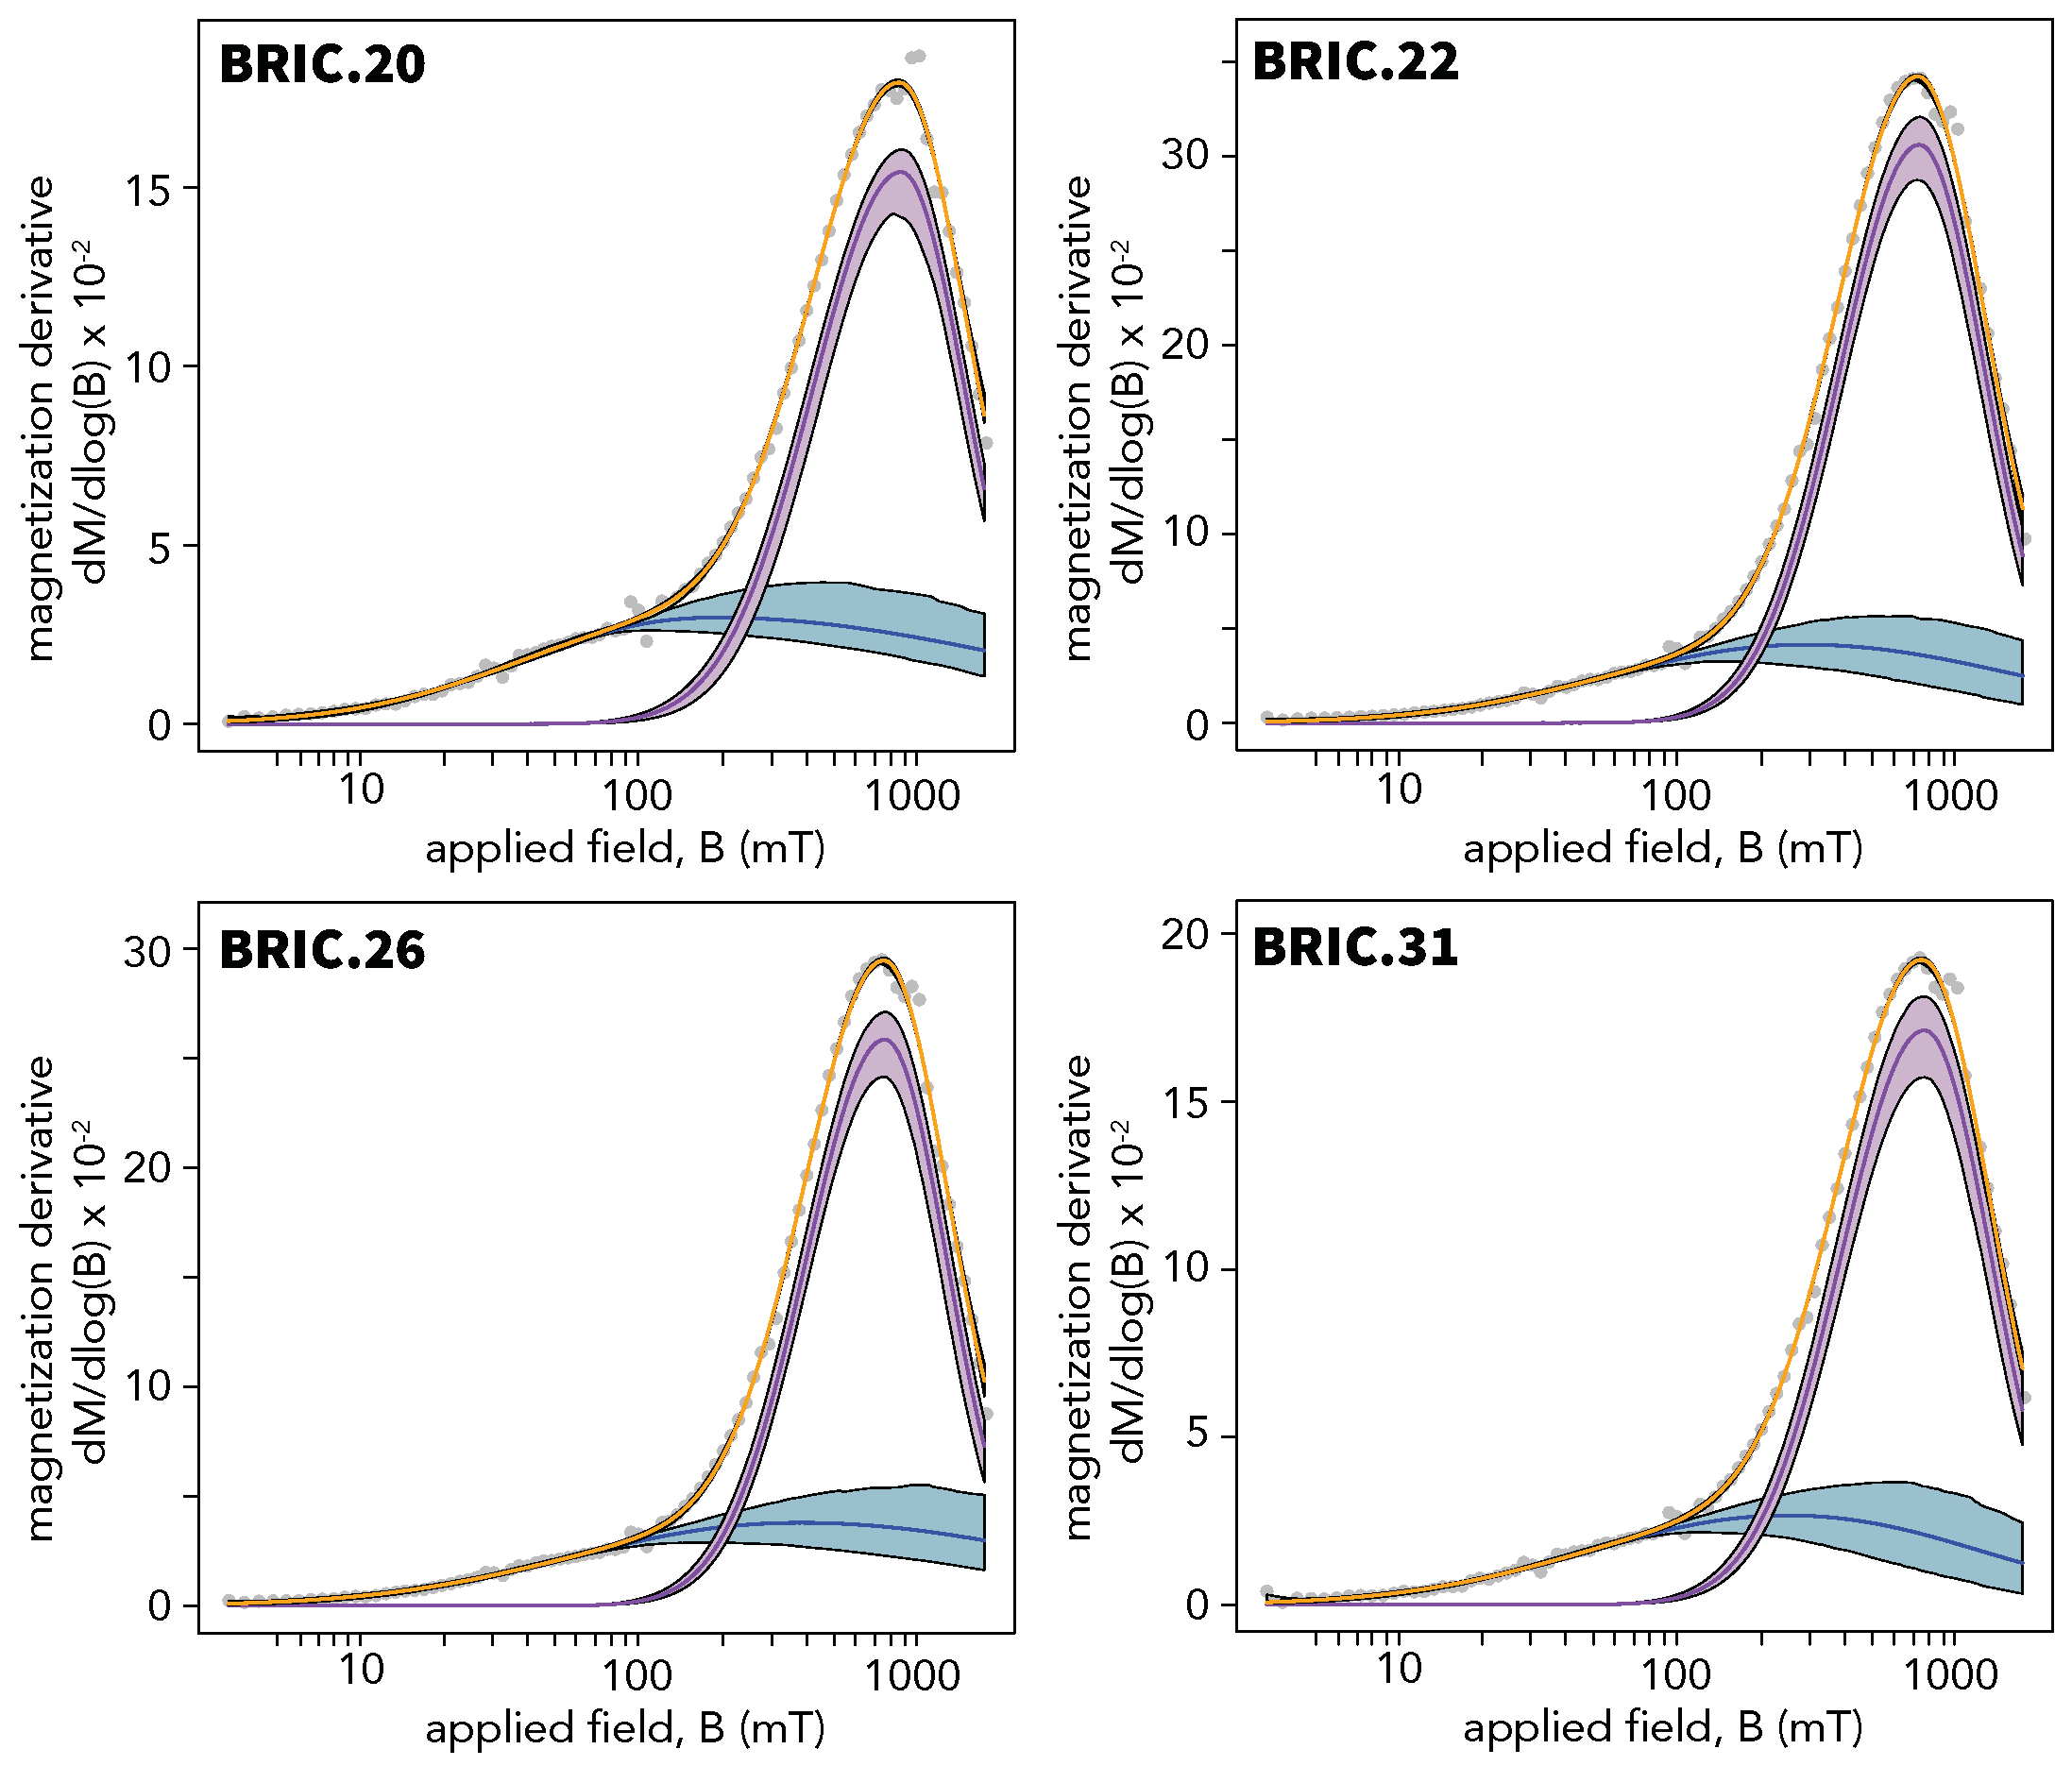
\includegraphics[width=0.9\textwidth]{figures/coercivity_spectra.pdf}
\caption{\small{Coercivity spectra developed from backfield demagnetization curves on BRIC intraclast specimens with the points being the data. The data were modeled using log-Gaussian functions implemented with the Max UnMix software package \citep{Maxbauer2016a} with the yellow curve corresponding to the model. The coercivity spectra can be well-explained with two distributions: the higher coercivity distribution in purple and the lower coercivity distribution in green.}}
\label{fig:coercivity_spectra}
\end{figure}

Backfield demagnetization curves, where the specimens were saturated in a 1.8 T field followed by a progressively larger field in the opposite direction, were developed on a Princeton Measurements vibrating sample magnetometer at the Institute for Rock Magnetism. Coercivity spectra, the derivative of the backfield curves, were modeled using the Max UnMix software package (\citealp{Maxbauer2016a}; Fig. \ref{fig:coercivity_spectra}). These spectra are well fit with two log-normal distributions associated with two populations of grains. One population has a median coercivity of $\sim$300 mT and a distribution that extends from the lowest to the highest coercivities (Fig. \ref{fig:coercivity_spectra}). The other population has a higher median coercivity of $\sim$700 mT and a coercivity distribution that is limited to the high coercivity range (Fig. \ref{fig:coercivity_spectra}). The median coercivity of the high-coercivity phase corresponds with the coercivity of single-domain hematite in the 300 nm to 10 $\mu$m range \citep{Ozdemir2014a}. The spread in coercivities associated with the lower coercivity population is consistent with these values down to those associated with finer-grained hematite; the coercivity of hematite becomes progressively lower for grains that are smaller than 300 nm in diameter \citep{Ozdemir2014a}.

\begin{figure}[!ht]
\noindent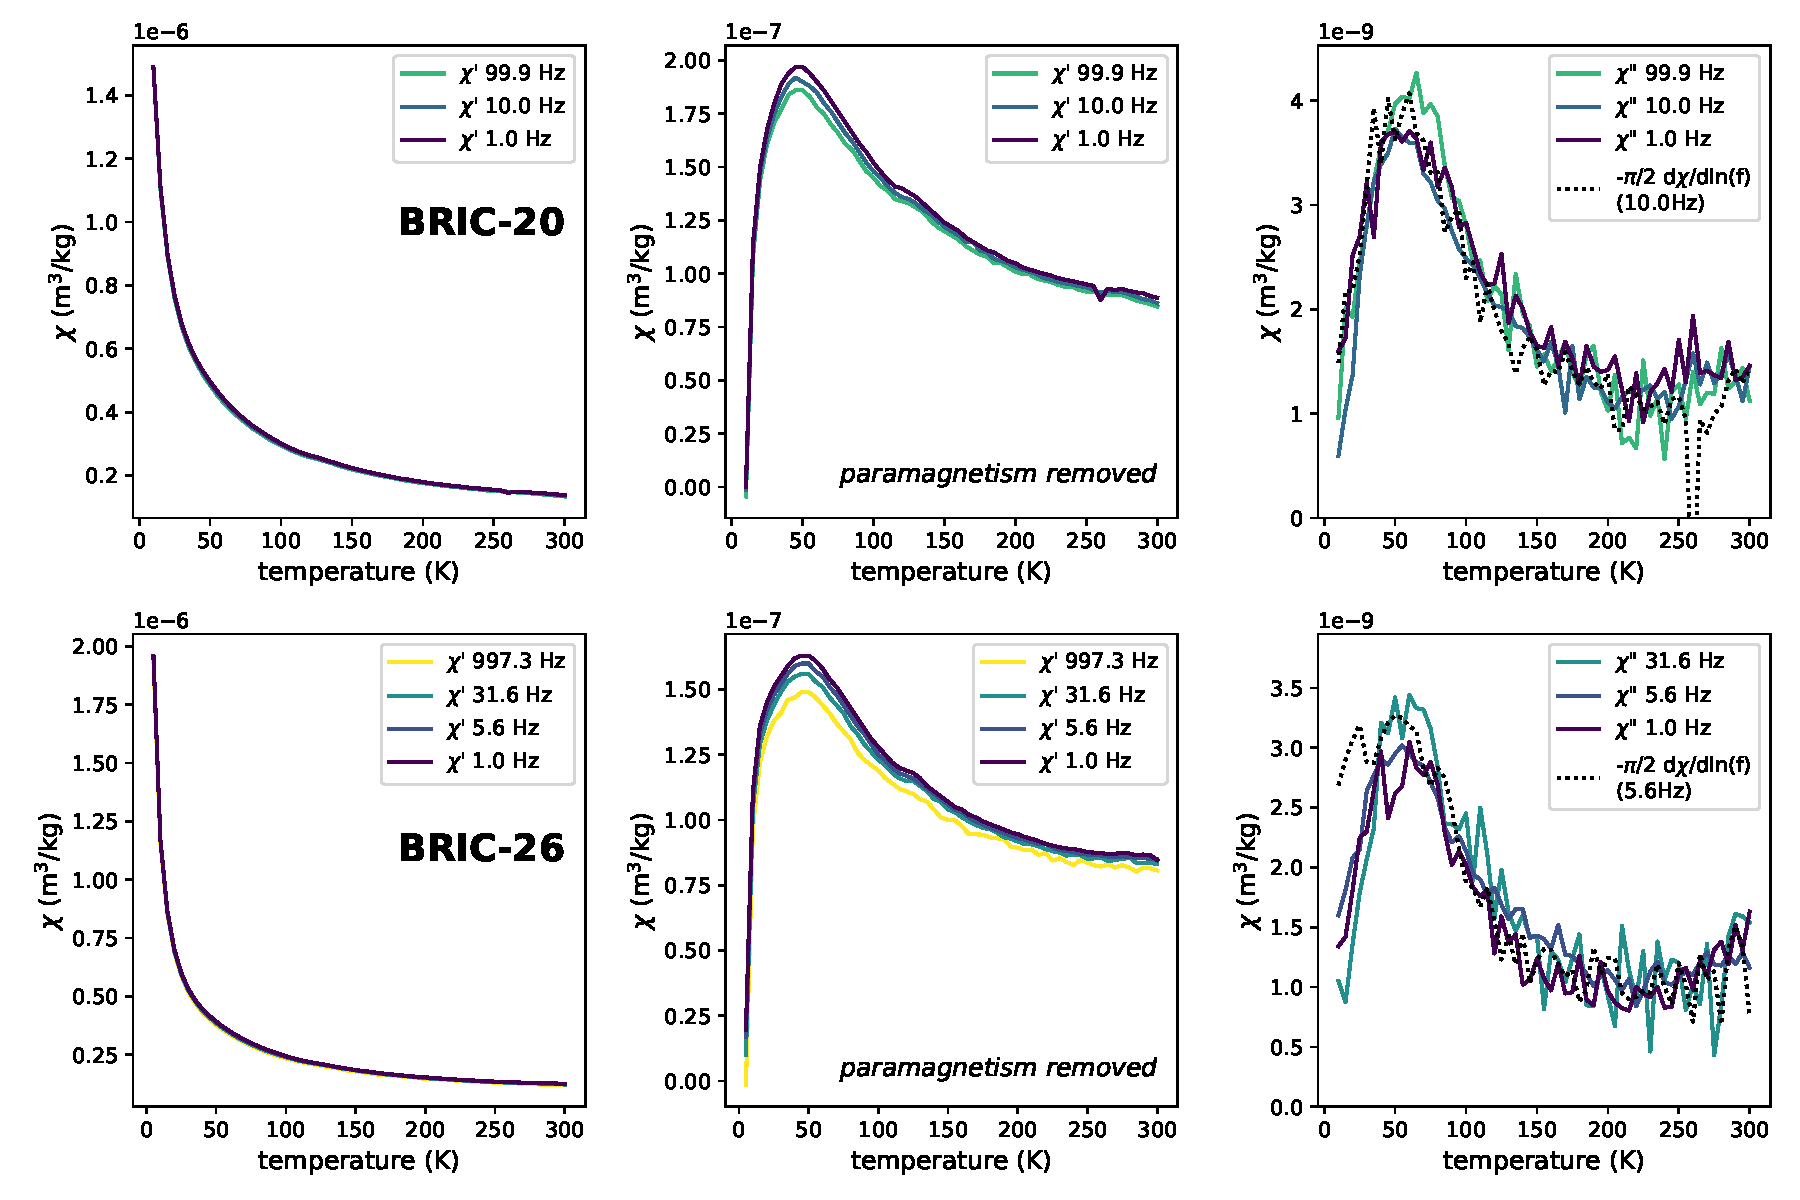
\includegraphics[width=\textwidth]{figures/low_temp_ac}
\caption{\small{Frequency and temperature dependence of magnetic susceptibility ($\chi$) for BRIC-20 and BRIC-26 from 10 to 300 K. The left panels show the in-phase susceptibility which is dominated by the paramagnetic component of the samples. In the middle panels, this paramagnetic component has been removed by creating a Curie-Weiss law model and subtracting it from the in-phase susceptibility data. Strong frequency dependence over the whole temperature range suggests a broad size distribution of nanoparticles (e.g. \citealp{Jackson2012a}). The right panels show the out-of-phase (quadrature) susceptibility as well as the $\pi/2$ relationship of $\chi''[viscosity] = -(\pi/2)(\partial \chi'/\partial lnf$) where $f$=frequency. These data document the presence of viscous superparamagnetic particles.}}
\label{fig:low_temp_ac}
\end{figure}

The frequency and temperature dependence of magnetic susceptibility was determined through experiments conducted on a Magnetic Properties Measurement System (MPMS) at the Institute for Rock Magnetism. The dependence of susceptibility on both temperature and frequency provides a sensitive and diagnostic means of characterizing magnetic nanoparticles \citep{Worm1999a}. We observe a frequency dependence of susceptibility that persists from 300 K down to 10 K (Fig. \ref{fig:low_temp_ac}). This frequency dependence can be attributed to viscous superparamagnetic grains whose magnetic viscosity has relaxation times comparable to the AC field reversal interval \citep{Worm1998a, Worm1999a}. This interpretation is supported by the frequency dependence of the in-phase susceptibility and the shared peak between the out-of-phase (quadrature) susceptibility and the $\pi/2$ law (\citealp{Mullins1973a}; Fig. \ref{fig:low_temp_ac}). That the frequency dependence extends across the full low-temperature range indicates a broad blocking temperature spectrum of viscous superparamagnetic grains associated with a wide size distribution of the nanoparticles. 

Hysteresis loops were measured from 5 T to -5 T on the MPMS at varying temperatures from room temperature (300 K) down to 50 K (Fig. \ref{fig:low_temp_loops}). These low-temperature hysteresis data reveal a progressive increase in remanent magnetization ($M_r$) as temperature decreases (Fig. \ref{fig:low_temp_loops}) leading to $M_r$ values that are between 9 and 13$\%$ higher at 50 K than at 300 K. This increase in $M_r$ at low temperatures is likely associated with superparamagnetic grains transitioning to behave as stable single domain grains at lower temperature. There is also an increase in saturation magnetization ($M_s$) as temperature decreases (Fig. \ref{fig:low_temp_loops}). However, the hysteresis loops require subtraction of a large paramagnetic component that becomes progressively non-linear at low temperatures leading to the possibility that this increase in $M_s$ is an artefact rather than an aspect of the ferromagnetic mineralogy of the samples. This increase in $M_r$ is insensitive to this correction and is therefore a more robust feature of the data. 

\begin{figure}[!ht]
\noindent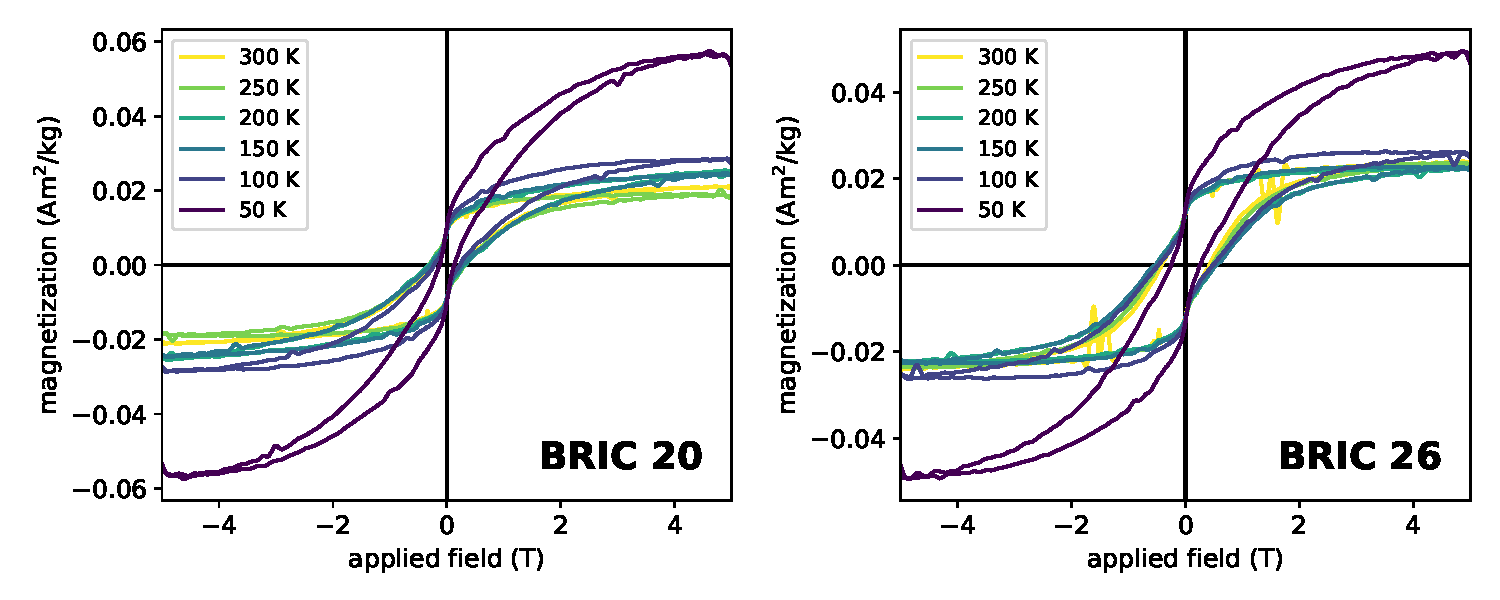
\includegraphics[width=\textwidth]{figures/low_temp_loops.pdf}
\caption{\small{Hysteresis loops measured from room temperature (300 K) down to 50 K for siltstone intraclast samples. The left panels are the raw uncorrected loops, the center panels remove the paramagnetic contribution using the methods of \citet{Jackson2010a} and the right panels zoom-in on applied fields close to 0 to illustrate the progressive increase in remanent magnetization ($M_r$) as temperature decreases.}}
\label{fig:low_temp_loops}
\end{figure}
 
M{\"o}ssbauer spectra were collected at the Institute for Rock Magnetism on bulk powders of intraclast samples at 300 K and 18 K (Fig. \ref{fig:mossbauer}). The main feature of these spectra is a magnetically split sextet with a magnetic hyperfine field of about 51.6 T -- diagnostic of hematite \citep{Dyar2006a}. Modeling of the spectra reveal that the majority of iron within the samples resides within hematite (58\% at 300 K and 60\% at 18 K). Due to the high-frequency of M{\"o}ssbauer spectroscopy, grains that are observed to be superparamagnetic at room temperature in typical rock magnetic experiments behave as stable ordered grains in M{\"o}ssbauer spectra. Nevertheless, there is a slight increase in the magnitude of the hematite sextet relative to the doublets in the 18 K spectrum, leading to the slight increase in modeled hematite content, likely associated with ordering of the smallest nanoparticles of hematite (\citealp{Bodker2000a}; Fig. \ref{fig:mossbauer}).

\begin{figure}[!ht]
\noindent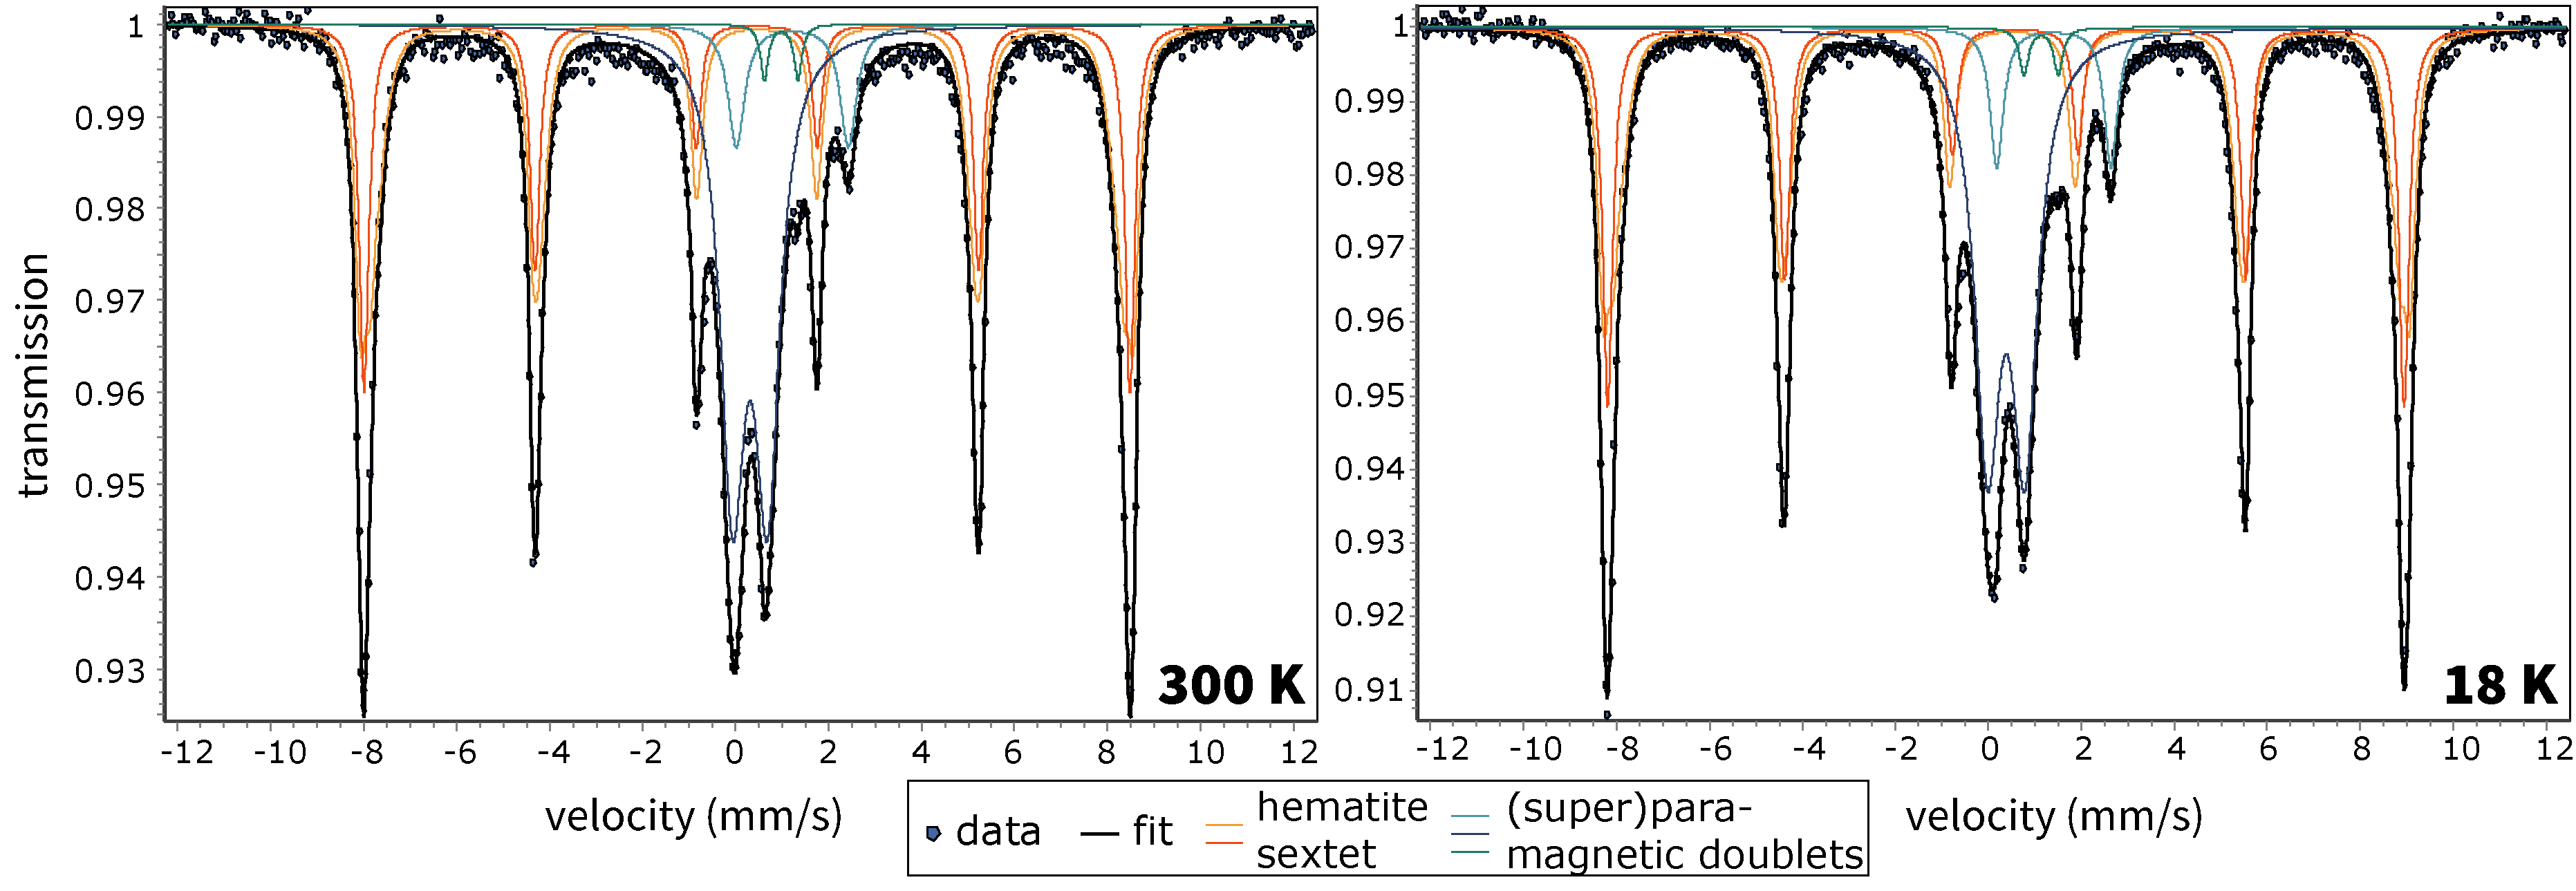
\includegraphics[width=\textwidth]{figures/mossbauer.pdf}
\caption{\small{M{\"o}ssbauer spectra developed at room temperature (300 K) and low temperature (18 K) on a powder of intraclast sample BRIC.22. Data are shown as dots with the black line representing a model fit. The sextet portion of the fit is shown with the red and yellow curves (representing the spread in hyperfine splitting resulting from a natural population) and is diagnostic of hematite. The central peak is comprised of doublets dominated by Fe$^{3+}$. The height of the hematite sextet relative to the central peak is slightly higher in the low temperature experiment likely due to ordering of the smallest hematite nanoparticles.}}
\label{fig:mossbauer}
\end{figure}

\section*{DISCUSSION}

Single-domain hematite grains have high coercivities ($>$150 mT; \citealp{Ozdemir2014a}) and high unblocking temperatures. As a result, populations of hematite within rocks are stable on long timescales, resistant to overprinting, and therefore attractive for paleomagnetic study. In contrast to magnetite, hematite grains retain stable single-domain behavior in crystals $>$1 $\mu$m with the threshold to multidomain behavior occurring when grain diameters exceed $\sim$100 $\mu$m \citep{Kletetschka2002a, Ozdemir2014a}. Hematite nanoparticles with diameters less than $\sim$30 nm have superparamagnetic behavior wherein thermal fluctuation energy overwhelms the ability of the grain to retain a stable magnetization at Earth surface temperatures \citep{Ozdemir2014a}. Given the scatter associated with experimental data (Fig. \ref{fig:summary}), the diameter associated with the superparamagnetic to stable single domain transition is slightly uncertain, but is on the order of 10s of nm \citep{Ozdemir2014a}. Regardless, hematite grains become progressively less influenced by thermal fluctuations as they reach grain sizes of a few hundred nanometers at which point they are stable up to temperatures approaching the N\'eel temperature of $\sim$685\textdegree C \citep{Swanson-Hysell2011a, Ozdemir2014a}. As a result, there is a strong relationship between grain volume and unblocking temperature that can be utilized to estimate grain size following N\'eel relaxation theory \citep{Neel1949a, Swanson-Hysell2011a}. A hematite population that is progressively unblocking at thermal demagnetization steps well below the N\'eel transition temperature, such as the mid-temperature component of the intraclasts, is comprised of grains within the $\sim$30 to $\sim$400 nm size range (Fig. \ref{fig:summary}). This fine-grain size is consistent with the pigmentary phase observed within the intraclasts (Fig. \ref{fig:intraclast_images}). 

Given the directional consistency of the mid-temperature component among the intraclasts (Fig. \ref{fig:intraclast_pmag}), this component must have dominantly formed as a chemical remanent magnetization after the intraclasts were redeposited in the channel. Chemical remanent magnetization acquisition by pigmentary hematite would have occurred as hematite grains grew to sizes above the superparamagnetic to stable single-domain transition resulting in the wide range of unblocking temperatures that is observed. The frequency dependence of susceptibility (Fig. \ref{fig:low_temp_ac}) and increase in remanent magnetization following saturation at low-temperature (Fig. \ref{fig:low_temp_loops}) both indicate the presence of a population of superparamagnetic grains. The coercivity spectra are consistent with a population of hematite that has a wide coercivity range extending from low coercivities up to high coercivities (the green component in the unmixing models of Fig. \ref{fig:coercivity_spectra}). Taken together and compared to the hematite coercivity compilation of \cite{Ozdemir2014a}, these data indicate that a population of authigenic hematite nanoparticles that spans from $<$30 nm to $>$300 nm is responsible for the post-depositional chemical remanent magnetization (Fig. \ref{fig:summary}). 

In contrast, the sharp unblocking temperature close to the N\'eel temperature of the high-temperature component indicates that it is dominantly held by hematite grains that are $>$400 nm (based on N\'eel relaxation theory; Fig. \ref{fig:summary}) such as the silt-sized hematite grains observed petrographically (Fig. \ref{fig:intraclast_images}). The high-coercivity population within the coercivity spectra (purple curves in Fig. \ref{fig:coercivity_spectra}) are consistent with this grain-size interpretation (Fig. \ref{fig:summary}). The high-temperature remanence component held by these grains was rotated along with the clasts indicating that it is primary and was acquired prior to the redeposition of the cohesive silt clasts. That this component is held by larger grains sizes supports it being a detrital remanent magnetization, rather than a chemical remanent magnetization that formed very early prior to clast erosion. 

Detailed rock magnetic data through the Nonesuch Formation, which immediately underlies the Freda Formation, reveal that the lacustrine lithologies preserve a depth-dependent environmental magnetic signature where the deep water facies have no hematite in contrast to hematite-rich shallow water facies in sediments of similar grain size \citep{Slotznick2018b}. This difference was interpreted by \citet{Slotznick2018b} as being due to microbial reductive dissolution of iron oxides at low oxygen levels in the deepest part of the lake and oxidation of the detrital input in the shallowest part of the lake. Sediment that was deposited at intermediate water depths within the lake contains both detrital magnetite and hematite with minimal evidence for post-depositional reduction or oxidation leading to an interpretation of intermediate oxygen levels \citep{Slotznick2018b}. That this depth-dependent relationship is consistent over significant length scales across the Midcontinent Rift basin indicates that hematite formation in those sediments, and likely the Freda Formation as well, is associated with redox conditions at the time of deposition rather than the subsequent migration of fluids. Oxidation of iron in surface environments often begins with the formation of fine-grained poorly crystalline ferrihydrite, which transforms to stable crystalline hematite at neutral pH on geologically short timescales \citep{Cudennec2006a, Jiang2018a}. The broad unblocking temperatures we observe for the chemical remanent magnetization in the Freda intraclasts are similar to those in hematite populations produced through experimental ferrihydrite to hematite conversion \citep{Jiang2015a}. The direction of this chemical remanence is distinct, but similar, to that of the detrital remanence with a change in both declination and inclination. This result suggests that the chemical remanence was acquired as plate motion continued at the end of the Keweenawan Track \citep{Swanson-Hysell2018a}. This chemical remanent magnetization direction is well-grouped (Fig. \ref{fig:insitu_pmag}) suggesting that the hematite that carries the remanence formed at a similar time rather than over a protracted period (which could lead to a streaked distribution; \citealp{Beck2003b}). One possibility is that the conversion from a phase associated with the ferrihydrite to hematite transition that formed in the sediments in the near-surface was thermally activated by the geothermal gradient as the sediments were buried. More than 4 km of Freda Formation sediments were deposited atop those investigated in this study within the thermally subsiding basin that would have led to protracted interval at temperatures $>$100 \textdegree C following deposition. Such thermal activation of the transition of ferrihydrite, and/or intermediary phases such as hydromaghemite, to hematite could explain the association of chemical remanence directions with burial within the Midcontinent Rift. This mechanism could also explain the association of authigenic hematite remanence with other types of tectonothermal events such as the well-documented syn-folding chemical remanence of the Mauch Chunk Formation that is associated with the Alleghanian orogeny \citep{Kent1985b, Opdyke2004a}.

\begin{figure}[!ht]
\noindent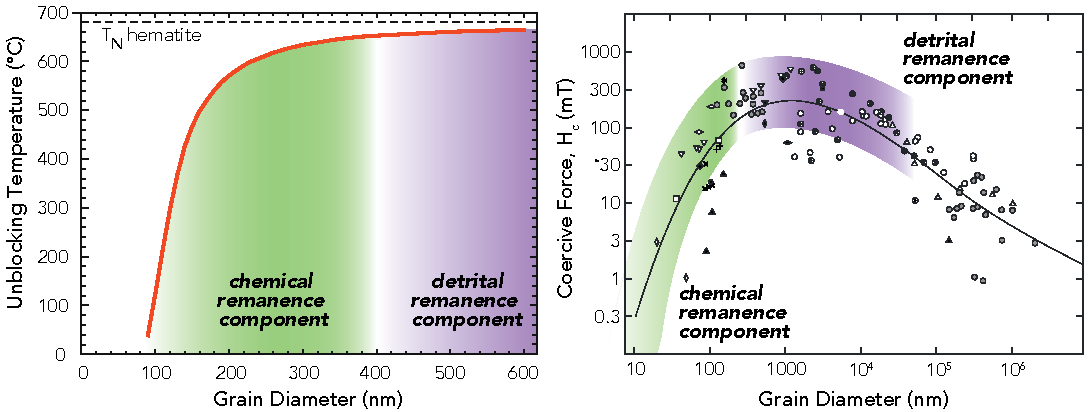
\includegraphics[width=\textwidth]{figures/component_summary.pdf}
\caption{\small{Left: Calculated unblocking temperatures using N\'eel thermal relaxation theory of idealized spherical hematite grains using a thermal fluctuation rate of 10$^{10}$ s$^{-1}$ and a relaxation time of 5 minutes for comparison to thermal demagnetization data (modified from \citealp{Swanson-Hysell2011a}). The unblocking temperatures of the mid-temperature chemical component (green) and the high-temperature detrital component (purple) are shown and can be used to infer grain size. The N\'eel transition temperature (T$_{\mathrm{N}}$) is shown with a dashed line. Right: Compilation of coercivity data from hematite as a function of grain diameter from \cite{Ozdemir2014a}. The higher coercivity population from Fig. \ref{fig:coercivity_spectra} corresponds to the larger grain sizes than the lower coercivity component associated with the chemical remanence.}}
\label{fig:summary}
\end{figure}

The differential unblocking temperature spectra of the two components within the Freda intraclasts provides strong support for the argument of \citet{Jiang2015a} that chemical and detrital remanent magnetization can be distinguished due to detrital remanence unblocking at the highest temperatures. However, the Freda intraclast data also show that while the detrital remanent magnetization can be well-isolated at temperatures as low as 650\textdegree C (specimen BRIC.31a in Fig. \ref{fig:intraclast_pmag}), the chemical remanent magnetization thermal unblocking spectra can overlap with that of the detrital remanence and extend up to temperatures closer to the N\'eel temperature (specimen BRIC.41a in Fig. \ref{fig:intraclast_pmag}). Therefore, to isolate primary remanence in red beds, best practice should be to proceed with very high resolution thermal demagnetization steps above 600\textdegree C, and particularly above 650\textdegree C. Characteristic remanence magnetization directions associated with hematite that are fit to components that span a wide range of unblocking temperatures including those lower than $\sim$650 \textdegree C are likely convolving a pigmentary chemical remanence and a detrital remanence held by larger grains. 

A complication with detrital remanent magnetization is associated inclination-shallowing -- an issue that has been explored in depth within the literature as pertains to hematite (e.g \citealp{Tauxe1984a, Bilardello2010a}). The presence of both pigmentary and detrital hematite complicates efforts that seek to use bulk magnetic fabrics to correct for these effects. This reality necessitates the use of careful methodologies that target the fabric of only the highest-unblocking-temperature hematite (e.g. \citealp{Bilardello2015a}) or that take other approaches such as analyzing the elongation of the directional distribution and correcting to values taken from secular variation models (the elongation-inclination method of \citealp{Tauxe2004a}).

Hematite-bearing sedimentary rocks have varied characteristics which has lead to the argument that it is difficult to apply results from red beds in one formation to those from another. However, the rock magnetic properties of the hematite grain size distributions that emerge from these data are associated with their mode of incorporation into the sediment. Hydrodynamic sorting associated with the delivery of detrital hematite will lead to a narrower and coarser size distribution of grains than that of authigenic pigmentary hematite growth. Authigenic growth can lead to a distribution of grains that span from sub-30 nm superparamagnetic grains up to stable single-domain grains $>$300 nm in diameter. Such an authigenic population has distinct rock magnetic characteristics including a very broad coercivity distribution and viscous superparamagnetic grains that can be detected through low-temperature magnetometry. 
 
Overall, the intraclast data, combined with those of the in-place siltstone, reveal that directional change at the highest unblocking temperatures provides an effective means to discriminate primary and secondary magnetizations within siltstones of the Freda Formation. The isolation of remanence carried by primary detrital hematite in $>$1 billion-year-old siltstones lends confidence to magnetostratigraphic records and paleogeographic interpretations that are based on interpretations of primary magnetization isolated from high-unblocking-temperature hematite in ancient red beds. 

%Text here ===>>>

%%

%  Numbered lines in equations:
%  To add line numbers to lines in equations,
%  \begin{linenomath*}
%  \begin{equation}
%  \end{equation}
%  \end{linenomath*}



%% Enter Figures and Tables near as possible to where they are first mentioned:
%
% DO NOT USE \psfrag or \subfigure commands.
%
% Figure captions go below the figure.
% Table titles go above tables;  other caption information
%  should be placed in last line of the table, using
% \multicolumn2l{$^a$ This is a table note.}
%
%----------------
% EXAMPLE FIGURE
%
% \begin{figure}[h]
% \centering
% when using pdflatex, use pdf file:
% \includegraphics[natwidth=800px,natheight=600px]{figsamp.pdf}
%
% when using dvips, use .eps file:
% \includegraphics[natwidth=800px,natheight=600px]{figsamp.eps}
%
% \caption{Short caption}
% \label{figone}
%  \end{figure}
%
% We recommend that you provide the native width and height (natwidth, natheight) of your figures.
% Specifying native dimensions ensures that your figures are properly scaled
%
%
% ---------------
% EXAMPLE TABLE
%
% \begin{table}
% \caption{Time of the Transition Between Phase 1 and Phase 2$^{a}$}
% \centering
% \begin{tabular}{l c}
% \hline
%  Run  & Time (min)  \\
% \hline
%   $l1$  & 260   \\
%   $l2$  & 300   \\
%   $l3$  & 340   \\
%   $h1$  & 270   \\
%   $h2$  & 250   \\
%   $h3$  & 380   \\
%   $r1$  & 370   \\
%   $r2$  & 390   \\
% \hline
% \multicolumn{2}{l}{$^{a}$Footnote text here.}
% \end{tabular}
% \end{table}

%% SIDEWAYS FIGURE and TABLE
% AGU prefers the use of {sidewaystable} over {landscapetable} as it causes fewer problems.
%
% \begin{sidewaysfigure}
% \includegraphics[width=20pc]{figsamp}
% \caption{caption here}
% \label{newfig}
% \end{sidewaysfigure}
%
%  \begin{sidewaystable}
%  \caption{Caption here}
% \label{tab:signif_gap_clos}
%  \begin{tabular}{ccc}
% one&two&three\\
% four&five&six
%  \end{tabular}
%  \end{sidewaystable}

%% If using numbered lines, please surround equations with \begin{linenomath*}...\end{linenomath*}
%\begin{linenomath*}
%\begin{equation}
%y|{f} \sim g(m, \sigma),
%\end{equation}
%\end{linenomath*}

%%% End of body of article

%%%%%%%%%%%%%%%%%%%%%%%%%%%%%%%%
%% Optional Appendix goes here
%
% The \appendix command resets counters and redefines section heads
%
% After typing \appendix
%
%\section{Here Is Appendix Title}
% will show
% A: Here Is Appendix Title
%
%\appendix
%\section{Here is a sample appendix}

%%%%%%%%%%%%%%%%%%%%%%%%%%%%%%%%%%%%%%%%%%%%%%%%%%%%%%%%%%%%%%%%
%
% Optional Glossary, Notation or Acronym section goes here:
%
%%%%%%%%%%%%%%
% Glossary is only allowed in Reviews of Geophysics
%  \begin{glossary}
%  \term{Term}
%   Term Definition here
%  \term{Term}
%   Term Definition here
%  \term{Term}
%   Term Definition here
%  \end{glossary}

%
%%%%%%%%%%%%%%
% Acronyms
%   \begin{acronyms}
%   \acro{Acronym}
%   Definition here
%   \acro{EMOS}
%   Ensemble model output statistics
%   \acro{ECMWF}
%   Centre for Medium-Range Weather Forecasts
%   \end{acronyms}

%
%%%%%%%%%%%%%%
% Notation
%   \begin{notation}
%   \notation{$a+b$} Notation Definition here
%   \notation{$e=mc^2$}
%   Equation in German-born physicist Albert Einstein's theory of special
%  relativity that showed that the increased relativistic mass ($m$) of a
%  body comes from the energy of motion of the body—that is, its kinetic
%  energy ($E$)—divided by the speed of light squared ($c^2$).
%   \end{notation}




%%%%%%%%%%%%%%%%%%%%%%%%%%%%%%%%%%%%%%%%%%%%%%%%%%%%%%%%%%%%%%%%
%
%  ACKNOWLEDGMENTS
%
% The acknowledgments must list:
%
% >>>>	A statement that indicates to the reader where the data
% 	supporting the conclusions can be obtained (for example, in the
% 	references, tables, supporting information, and other databases).
%
% 	All funding sources related to this work from all authors
%
% 	Any real or perceived financial conflicts of interests for any
%	author
%
% 	Other affiliations for any author that may be perceived as
% 	having a conflict of interest with respect to the results of this
% 	paper.
%
%
% It is also the appropriate place to thank colleagues and other contributors.
% AGU does not normally allow dedications.


\acknowledgments
This research was supported by the Esper S. Larsen, Jr. Research Fund and the National Science Foundation through grant EAR-1419894. Rock magnetic experiments were conducted on a visiting fellowship at the Institute for Rock Magnetism which is made possible through the Instrumentation and Facilities program of the National Science Foundation, Earth Science Division and funding from the University of Minnesota. SPS was supported by the Miller Institute for Basic Research in Science. The Wisconsin Department of Natural Resources granted a research and collection permit that enabled sampling within Copper Falls State Park. Oliver Abbitt assisted with field work, Taiyi Wang assisted with paleomagnetic analyses and Tim Teague provided technical support for EBSD analyses. Peat Solheid, Mike Jackson, and Dario Bilardello provided technical support at the Institute for Rock Magnetism. Discussions with them, and with Josh Feinberg and Bruce Moskowitz, provided insight on rock magnetic data interpretation. Reviews from Associate Editor Mark Dekkers, Dario Bilardello and an anonymous referee improved the manuscript. Data associated with this study are available within the MagIC database and a Github repository associated with this work.


%% ------------------------------------------------------------------------ %%
%% References and Citations

%%%%%%%%%%%%%%%%%%%%%%%%%%%%%%%%%%%%%%%%%%%%%%%
% BibTeX is preferred:
%
\bibliography{../../references/allrefs}
%
% don't specify bibliographystyle
%%%%%%%%%%%%%%%%%%%%%%%%%%%%%%%%%%%%%%%%%%%%%%%



% Please use ONLY \citet and \citep for reference citations.
% DO NOT use other cite commands (e.g., \cite, \citeyear, \nocite, \citealp, etc.).
%% Example \citet and \citep:
%  ...as shown by \citet{Boug10}, \citet{Buiz07}, \citet{Fra10},
%  \citet{Ghel00}, and \citet{Leit74}.

%  ...as shown by \citep{Boug10}, \citep{Buiz07}, \citep{Fra10},
%  \citep{Ghel00, Leit74}.

%  ...has been shown \citep [e.g.,][]{Boug10,Buiz07,Fra10}.


\end{document}



More Information and Advice:

%% ------------------------------------------------------------------------ %%
%
%  SECTION HEADS
%
%% ------------------------------------------------------------------------ %%

% Capitalize the first letter of each word (except for
% prepositions, conjunctions, and articles that are
% three or fewer letters).

% AGU follows standard outline style; therefore, there cannot be a section 1 without
% a section 2, or a section 2.3.1 without a section 2.3.2.
% Please make sure your section numbers are balanced.
% ---------------
% Level 1 head
%
% Use the \section{} command to identify level 1 heads;
% type the appropriate head wording between the curly
% brackets, as shown below.
%
%An example:
%\section{Level 1 Head: Introduction}
%
% ---------------
% Level 2 head
%
% Use the \subsection{} command to identify level 2 heads.
%An example:
%\subsection{Level 2 Head}
%
% ---------------
% Level 3 head
%
% Use the \subsubsection{} command to identify level 3 heads
%An example:
%\subsubsection{Level 3 Head}
%
%---------------
% Level 4 head
%
% Use the \subsubsubsection{} command to identify level 3 heads
% An example:
%\subsubsubsection{Level 4 Head} An example.
%
%% ------------------------------------------------------------------------ %%
%
%  IN-TEXT LISTS
%
%% ------------------------------------------------------------------------ %%
%
% Do not use bulleted lists; enumerated lists are okay.
% \begin{enumerate}
% \item
% \item
% \item
% \end{enumerate}
%
%% ------------------------------------------------------------------------ %%
%
%  EQUATIONS
%
%% ------------------------------------------------------------------------ %%

% Single-line equations are centered.
% Equation arrays will appear left-aligned.

Math coded inside display math mode \[ ...\]
 will not be numbered, e.g.,:
 \[ x^2=y^2 + z^2\]

 Math coded inside \begin{equation} and \end{equation} will
 be automatically numbered, e.g.,:
 \begin{equation}
 x^2=y^2 + z^2
 \end{equation}


% To create multiline equations, use the
% \begin{eqnarray} and \end{eqnarray} environment
% as demonstrated below.
\begin{eqnarray}
  x_{1} & = & (x - x_{0}) \cos \Theta \nonumber \\
        && + (y - y_{0}) \sin \Theta  \nonumber \\
  y_{1} & = & -(x - x_{0}) \sin \Theta \nonumber \\
        && + (y - y_{0}) \cos \Theta.
\end{eqnarray}

%If you don't want an equation number, use the star form:
%\begin{eqnarray*}...\end{eqnarray*}

% Break each line at a sign of operation
% (+, -, etc.) if possible, with the sign of operation
% on the new line.

% Indent second and subsequent lines to align with
% the first character following the equal sign on the
% first line.

% Use an \hspace{} command to insert horizontal space
% into your equation if necessary. Place an appropriate
% unit of measure between the curly braces, e.g.
% \hspace{1in}; you may have to experiment to achieve
% the correct amount of space.


%% ------------------------------------------------------------------------ %%
%
%  EQUATION NUMBERING: COUNTER
%
%% ------------------------------------------------------------------------ %%

% You may change equation numbering by resetting
% the equation counter or by explicitly numbering
% an equation.

% To explicitly number an equation, type \eqnum{}
% (with the desired number between the brackets)
% after the \begin{equation} or \begin{eqnarray}
% command.  The \eqnum{} command will affect only
% the equation it appears with; LaTeX will number
% any equations appearing later in the manuscript
% according to the equation counter.
%

% If you have a multiline equation that needs only
% one equation number, use a \nonumber command in
% front of the double backslashes (\\) as shown in
% the multiline equation above.

% If you are using line numbers, remember to surround
% equations with \begin{linenomath*}...\end{linenomath*}

%  To add line numbers to lines in equations:
%  \begin{linenomath*}
%  \begin{equation}
%  \end{equation}
%  \end{linenomath*}



